\documentclass[11pt,a4paper]{report}
\usepackage[margin=1.5in]{geometry}
\usepackage{amsmath}
\usepackage{array}
\usepackage{caption}
\usepackage[hidelinks]{hyperref}
\usepackage{subcaption}
\usepackage{setspace}
\usepackage{fixltx2e}
\usepackage[superscript]{cite}
\usepackage[pdftex]{graphicx}
\graphicspath{{assets/}}

\usepackage{graphicx}
\usepackage{amsmath,amssymb,latexsym}
\usepackage{float}
\usepackage{subcaption}


\usepackage{listings}
\usepackage{color}
\definecolor{lightgray}{rgb}{.9,.9,.9}
\definecolor{darkgray}{rgb}{.4,.4,.4}
\definecolor{purple}{rgb}{0.65, 0.12, 0.82}

\lstdefinelanguage{JavaScript}{
  keywords={typeof, new, true, false, catch, function, return, null, catch, switch, var, if, in, while, do, else, case, break},
  keywordstyle=\color{blue}\bfseries,
  ndkeywords={class, export, boolean, throw, implements, import, this},
  ndkeywordstyle=\color{darkgray}\bfseries,
  identifierstyle=\color{black},
  sensitive=false,
  comment=[l]{//},
  morecomment=[s]{/*}{*/},
  commentstyle=\color{purple}\ttfamily,
  stringstyle=\color{red}\ttfamily,
  morestring=[b]',
  morestring=[b]"
}

\lstset{
   language=JavaScript,
   backgroundcolor=\color{lightgray},
   extendedchars=true,
   basicstyle=\footnotesize\ttfamily,
   showstringspaces=false,
   showspaces=false,
   numbers=left,
   numberstyle=\footnotesize,
   numbersep=9pt,
   tabsize=2,
   breaklines=true,
   showtabs=false,
   captionpos=b
}


\newcommand{\HRule}{\rule{\linewidth}{0.5mm}}
\renewcommand*{\sectionautorefname}{Section}
\renewcommand*{\subsectionautorefname}{Section}
\renewcommand*{\subsubsectionautorefname}{Section}

\def\bsq#1{%both single quotes
\lq{#1}\rq}
\def\f0{f\textsubscript{0}}
\onehalfspacing

\begin{document}

\begin{titlepage}
    \begin{center}
        \large Computing BEng \\[0.5cm]
        \large Individual Project \\[0.5cm]
        \HRule \\[0.4cm]
        {\huge \bfseries Rubato: An Adaptive Musicality Tutor using Pitch Detection \\[0.4cm]}
        \HRule \\[1.5cm]
            \begin{flushleft}
                \large               
                Conrad \textsc{Godfrey}\\
            \end{flushleft}
            \begin{flushright}
                \large
                \emph{Supervisor:}\\
                Iain \textsc{Phillips}
            \end{flushright}
        \vfill
        {\large \today}
    \end{center}
\end{titlepage}


\begin{abstract}
In this project, we propose an adaptive learning web application that employs pitch detection algorithms. As web based learning is growing more and more popular, an increasing number of companies are adopting adaptive learning into their education models, most notably, Duolingo, a language tutoring website. There exists, however, no such application of this type in the domain of music theory, though there are many non-adaptive websites that attempt to teach it. With the advent of HTML5 and the Web Audio API, an opportunity also exists to run browser based pitch detection algorithms to analyse various aspects of a pupil's musical ability, yet there are currently no browser based pitch detection algorithms suitable for measuring vocal performance. We devise a highly robust, fast algorithm suitable for measuring sung pitch in pupils wishing to measure their tuning, and we apply this in an adaptive learning context.
\end{abstract}


\renewcommand{\abstractname}{Acknowledgements}
\begin{abstract}
I would like to thank my supervisor Iain Phillips for his continued support and guidance throughout my project. I would also like to thank my friends and family for their company for the past three years at Imperial College. A big thank you is also due to those who helped me pitch detect my algorithm, David Maguire, Elise van Lil, Alex Moore, Emily Ooi, and Tom Watkins.

\end{abstract}
\tableofcontents
%\listoffigures
%\listoftables
\chapter{Introduction}

\par In this paper I propose an application to harness the power of the modern web browser to deliver engaging musicality tutoring based on adaptive learning principles. The application will comprise of various exercises designed to challenge and improve a user's musicality, and keep track of their progress as well as adapt to their strengths and weaknesses in different areas.
\vspace{1em}
\par

\section{Adaptive learning}
As usage of the world wide web has become ubiquitous among citizens of the developed world, web based teaching has grown rapidly to try and modernize learning methods to fit into the 21st century lifestyle. Increasing numbers of companies like Coursera\cite{coursera}, Codeacademy\cite{codeacademy}, Duolingo\cite{duolingo} are providing easily accessible education for anyone with an internet connection and a desire to learn. Codeacademy and Duolingo in particular are notable for their use of rich, highly interactive learning tools which - through requiring the user to have an input into the educational process - establish a feedback system with powerful results\cite{vesselinov2012duolingo}. These companies offer a variety of different programmes the user can study, and each of these is taught through a series of exercises, the results of which are used to track the users progress through the course, and provide statistics on how much they have learned. Duolingo, a website that teaches foreign languages, takes it a step further by introducing adaptive learning methods to recognise the user's proficiency in various areas, information it can then use to tailor-make lessons to fit the user's needs. Duolingo is arguably the best best-known example of an adaptive learning system put into practice. It will therefore often be used for comparison throughout this report, as it has also provided a lot of inspiration for my thinking about the direction my project will take.

\begin{figure}
	\centering
	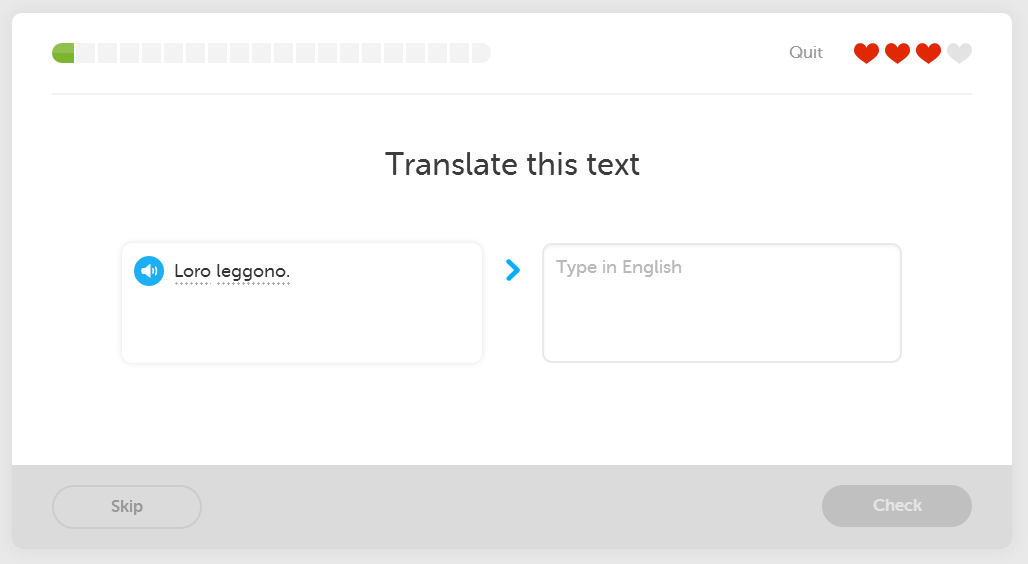
\includegraphics[scale=0.5]{duolingo.png}
	\caption{Duolingo adapts the questions it asks depending on the user's strengths and weaknesses}
\end{figure}

\section{Music teaching on the web}

\vspace{1em}
\par
The web is a great place to train the musical ear, a skill we shall refer to under the term of \bsq{musicality} from hereon in. The rich media options possible on modern day web browsers mean that the input and output of music to a web browser is not only easy to implement, but easy to make user friendly. However, while there are many \bsq{music theory tutors} and \bsq{ear trainers} available, there are no existing adaptive learning solutions. Such a solution would hopefully be invaluable to potential learners as the current best solutions still have no idea who you are and what you've achieved after you leave the page.
\par
In order to teach adaptively we must analyse information about a user's performance, and then change how we teach accordingly. 
There are various ways of measuring musicality, which will be discussed in more detail later, and we will rely on these metrics to adapt the learning experience to fit the user.

\section{Pitch detection}
There are very few examples of pitch detection algorithms running in browser, and the few that there are aren't very useful to a singer\cite{webaudiodemos,audioStretch}. This is because they all try to perform real-time pitch detection where the output is calculated at the same time the user is singing. This is useful for instruments like guitars where when you strike a note, you can be assured it will remain fairly constant in pitch, but the human voice is prone to slight variations in pitch that can cause a real-time algorithm to oscillate around a point, making it hard to gauge what the note you actually sung was. It is with this in mind that I aim to create a meaningful pitch detection algorithm that looks at a 2-3 second audio sample and gives the user accurate pitch data for that period

\section{Existing work}


\section{Objectives}

I aim to build a program that can successfully teach musicality. To ensure I achieve this goal, the following criteria must be met:
	\begin{itemize}
		\item \textbf{Adaptive} - The product must analyse the user's progress and their strengths, and adopt the content of their learning experience accordingly. This will require a user account system, as well as intelligent handling of the exercise data they generate.
		\item \textbf{Intuitive} - The product must be simple to use, and the exercises given to the user must be simple to understand, even for a beginner.
		\item \textbf{Engaging} - The user must want to learn and continue learning. In a study of Duolingo's effectiveness, 93.8\% of participants intended to continue using the website after the study had finished \cite{griffiths2012profile}. I would like to aim for at least 75\%.
		\item \textbf{Pitch Recognition} - Another way I'm aiming push the boundaries of musicality teaching is through introducing exercises that involve pitch data to be submitted by the user, and then grade them based on how accurate they are.
	\end{itemize}
\chapter{Background}
	\section{Adaptive learning}
	Web based learning has been a topic of interest almost since the birth of the web\cite{alexander1995teaching}, and the introduction of the HTML5 standard has opened up even more opportunities for computers to play a role in the education process\cite{griffiths2012profile}. 3 notable examples of web based learning systems (WLS) are:
	\begin{itemize}
		\item Coursera, a site that provides lecture material for various university level courses.
		\item  Codeacademy, a site designed to help people learn coding by getting them to undertake interactive browser based programming lessons.
		\item and Duolingo, a site designed to help the user learn foreign languages through interactive exercises that tries to tailor-make each exercise to the users needs by analysing their strengths/weaknesses.
	\end{itemize}
	The end aim of these sites is the same as all WLS's: to educate the user, but there are key differences between them which we can use to categorise them further into a hierarchy.
	\begin{itemize}
		\item Coursera is a \emph{static} WLS, it allows a one way interaction whereby the user can view/download learning material. While this is surely useful, it is really the base level of what a WLS can do.
		\item Codeacademy is a \emph{dynamic} WLS, it allows a two way interaction that introduces feedback for the user, enhancing the learning experience beyond a static WLS.
		\item Duolingo is an \emph{adaptive} WLS, it includes all the features of a dynamic WLS, only it can treat every user differently by analysing their strengths and weaknesses \cite{duolingoDataDriven}. This adaptive approach allows for superior teaching to static or dynamic WLS's, as if implemented correctly it will start to mimic the tailor-made learning experience one might receive from a real-world \bsq{for-hire} tutor.
	\end{itemize}
	
	
	\subsection{Adaptive learning in music}
		There are many ways that adaptive learning techniques can be applied in a musical context. As an example, imagine a simple exercise.
		\begin{itemize}
			\item The user is played a rhythmical phrase.
			\item They must then replicate the phrase by tapping it in on the space bar. 
			\item The application then calculates how accurate the user's approximation of the rhythm is, and feeds this information back to the user
		\end{itemize}
		After repeating this exercise multiple times the application notices something: The user is always getting examples featuring multiple consecutive dotted quavers wrong		\footnote{This is a type of rhythm that could prove difficult for the user as it can sound like the rhythm is going in and out of time due to it's naturally syncopated nature 		against a four four baseline}, and determines that this particular rhythmical device is something the user is struggling with. It can then subtly adapt future exercises to 	incorporate this device prominently, in order to expose the user to it as much as possible, and hopefully cause them to improve their understanding of that specific rhythm, and rhythm in general.
	\section{Platform choice}
	As the modern internet browser has become more and more powerful, web apps have been able to reduce the previous speed disadvantages they faced when compared with their native equivalents. The web-platform is advantageous due to having a singular codebase, meaning that it can be used by anyone with a web browser, independent of their device, so it has the potential to reach more users. Another key advantage of building a web app is that as user testing is so key to evaluating the app's success, when the time comes, and I want to show it to users, I can easily point people to my website and people will know how to get to it. Distributing a mobile app to others for testing purposes is painful, and difficult to update once they have installed it, with a web app I can instantly change the build of my website, and my aunt who's testing it in Jamaica won't have to do anything more than refresh the page.
	\section{Existing Musicality Tutors}
	
	There are a wide variety of existing web-based applications that teach musicality, to varying degrees. There are programs to allow you to practice interval recognition\cite{intervalEarTrainer}, identify a note in a chord, practice recognition of rhythms\cite{rhythmTrainer}. A lot of these programs are standalone, and focussed on one specific area. Musictheory.net\cite{musicTheorynet} is a good example of a website that that goes beyond that, it provides exercises that test a wide variety of skills, trains your ear as well as providing music theory lessons. However Musictheory.net provides no adaption to the user, the furthest it goes is allowing you to specify what you want to be taught, but it is not intelligent enough to work it out itself.
	\section{Music Theory}
	In order to understand some of the workings of the program it will be necessary to delve briefly into a little music theory. We will examine the fundamentals of Western music theory, as well as theory of pitch. From here on we shall talk exclusively in terms of Western music theory, as it is the theory that the overwhelming majority of contemporary Western music is based upon.
	

	\subsection{Pitch}
	\par The fundamental quality of a note played on the piano, plucked on the guitar, or sung by the voice is it's pitch. The other defining quality of a note is it's timbre/tone i.e. whether it sounds harsh or mellow, buzzy or clean, but this is a quality that is very hard to quantify, and also not as important to the overall melody of a piece of music - The same melody played on a guitar and a piano can certainly be considered to be the same piece of music, despite the differing tones of the instruments, but if you change the pitch of any notes, it becomes a different melody entirely. So of an individual note in a melody, we can say that it's pitch is it's defining characteristic.
	
	\par What do we mean by pitch? Scientifically, the pitch value of an audio signal is determined by that signal's fundamental frequency, \f0, where a higher frequency corresponds to a higher pitch, and a lower frequency a low pitch, however in terms of human perception, it is not as concrete as this, as there are various different psychoacoustic phenomena that determine how "high" or "low" a given note sounds. For example, a sinusoidal tone played at the same frequency at a low volume followed by a high volume will appear to be playing 2 different pitches, with the louder tone sounding lower in pitch. However, sinusoidal tones are much simpler than the rich complex tones of a musical instrument, which due to being constructed of many different frequencies can provide the listener with more cues as to the pitch they are at, so for the purposes of this project we will define pitch as it is defined in most musical contexts, as a logarithmic function of frequency.	
	
	\par Some instruments like pianos and guitars have predetermined pitches that the instrumentalist can produce. Others, like the violin or human voice, can create any pitch within a given spectrum in a continuous fashion. These two classes of instrument are quite different in that the latter type requires a more precise ear to play so that they sound in tune.
	
	\subsubsection{The Scale}
	There are of course an infinite number of pitches, as there are infinitely many different frequencies that an audio signal can have. However, if you start from a base frequency and gradually increase the pitch, you will eventually find that the note \bsq{sounds the same} as the note you started on, only higher. This happens every time you double the frequency, a ratio called an \bsq{octave}, and is an interesting property of the ear. Thus in the range of an octave, you can find all the pitches you could possibly think of. For the purposes of making music though, these pitches are quantised into 12 different notes. They are recognisable on the musical keyboard as shown below. The \bsq{\#} and \bsq{b} characters denote a sharpening or flattening of a pitch, i.e. a raising or lowering of the pitch respectively.
	
	\begin{figure}[h]
		\centering
		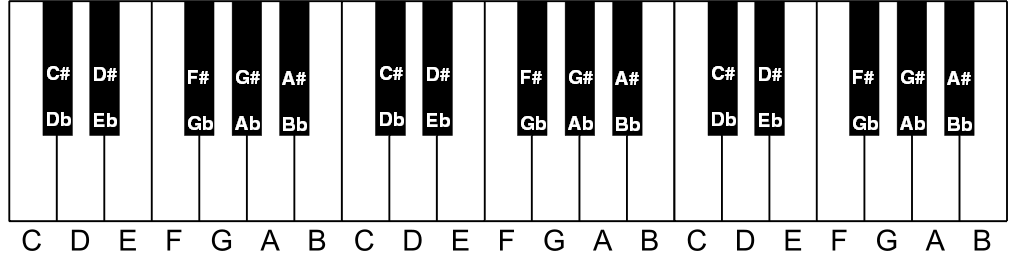
\includegraphics[scale=0.5]{keyboard.png}
		\caption[Caption]{The 12 notes of the Western scale. License\footnote{This file is licensed under the Creative Commons Attribution-Share Alike 2.5 Generic license, Author: Tobias R}}
	\end{figure}
	
	\subsubsection{Representing pitch}
	We now know about the 12 different notes in the Western scale, but as we have mentioned, simply knowing that a note's pitch is a \bsq{C} doesn't give us complete information about the note, as we are missing the octave information that tells us how high or low the note is. In this report, there are two main representations we will use.
	\begin{itemize}
		\item \textbf{Scientific notation} : This works on the basis that \bsq{middle C}, the C in the middle of a normal piano, is represented as C4. The next note above that is C\#4 or Db4, followed by D4 and so on until we reach B4, 11 semitones up. The next note after this is the C again, and since we have completed a full octave, we denote it C5. Similarly going downwards, the note directly below C4 is B3 etc. all the way down to C3, where the pattern repeats. This is arguably the most intuitive way of representing both a pitch and an octave as concisely as possible.
		\item \textbf{MIDI notation} :  This is the format used to store MIDI data, the most widely used music sequencing data format. It works on the principle that middle C is represented by the number 60, and incrementing and decrementing this number gives you the notes a semitone either side. This is convenient as it allows us handle the numerical side  of musical analysis with ease.
	\end{itemize}
	
	\subsubsection{Tuning}
	Tuning defines the mapping between frequency and notes. Convention dictates that the A above middle C on a piano (A4 in scientific notation or 69 in MIDI) is tuned at 440Hz (this is where the 440 comes from in the equation above), and this is referred to as \bsq{tuning to A440}. In \bsq{Equal Temperament}, the tuning system found in most modern pianos, all notes are spaced equally, which means that you can play in any key and still produce the same sound. In equal temperament:

	\begin{itemize}
		\item Doubling the frequency causes an increase in pitch of an octave, so A880 is the next A above A440.
		\item Since a leap of 12 semitones is caused by a doubling of the \f0 , it follows that the frequency ratio between each semitone (any two adjacent notes on the keyboard above) is \(2^\frac{1}{12}\) or about \(1.059\).
	\end{itemize}
	
	
	\subsubsection{Converting from frequency to pitch}
	
	For the purposes of this program it will often be necessary to convert between frequency and pitch. Using equal temperament and the MIDI notation, we can define a function thus.
	
		\[p=69+12\times {\log_2 \frac{f}{440Hz}}\] 
		
	where \(p\) is the pitch in MIDI notation, and \(f\) is the frequency.
	
	As mentioned previously in the section regarding the scale, there are only 12 different notes that are commonly used, yet this function can provide us with fractional values. What sense can we make of a number like 54.38? The unit most commonly used to represent fractions of a semitone is the cent. There are 100 cents in a semitone, so the number 54.38 would be translated to a F\#3 at 38 cents sharp.
	
	\subsubsection{Intervals}
	An interval is the distance between two notes as measured by the ratio of their frequencies. We have discussed one interval already, that being the octave, who's frequency ratio is 2:1. The next simplest interval is the \bsq{perfect fifth}, who's frequencies have a ratio of 3:2. Now we run into a problem with equal temperament. While the perfectly spaced notes of the piano are useful for their flexibility with respect to what key you wish to play in, they cannot accurately represent the purest intervals such as the perfect fifth. The closest interval on the piano is 7 semitones, or a ratio of \(2^\frac{7}{12}\):1 = 1.4983. Thankfully however, this slight difference is not great enough to offend most peoples' ears.
	\par The nature of an interval is such that two intervals starting on different notes will have a similar sound. Taken out of any harmonic context, an interval of a perfect fifth starting on an A will have the exact same effect as one starting on a C, or F, or any other note. This is why if you play a piece in a different key to that which it was written (meaning all the notes are shifted down or all are shifted up from where they should be) you can still call it the same piece, and indeed it will still very recognisably be the same piece, as all of the intervals in the accompaniment and melody will be the same).
	\subsubsection{The importance of good intonation}
	\par For instrumentalists of the continuously pitched instruments mentioned above such as the violin and human voice, producing correctly tuned intervals is a vital skill known as "intonation". Poor intonation can be the downfall of many a chamber choir, or ensemble, as one person singing wrong notes can lead half the group into another key which will sound very jarringly unpleasant. What's more, good sight reading depends on the ability to not only tune the intervals correctly, but to be able to recall what they sound like, and translate written music directly into performance in real time. Within the classical singing circuit, good sight reading is one of the most desirable, and rare, qualities in a singer, and a good sight reader can command high fees for their time.
	\begin{figure}[h]
		\centering
		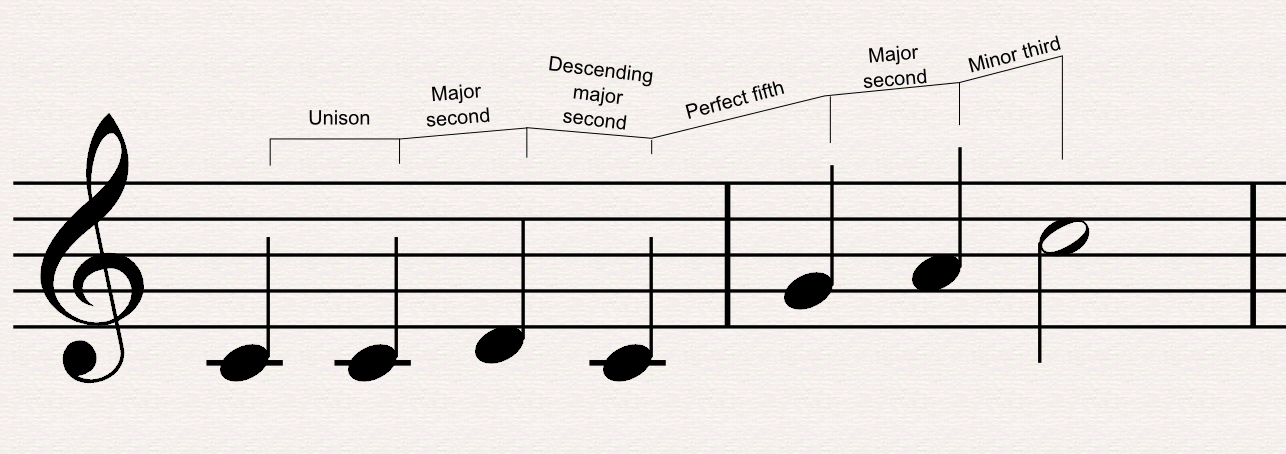
\includegraphics[scale=0.4]{intervals.png}
		\caption{Any given melody can be thought of as a sequence of intervals}
	\end{figure}		
	
	\par Practising intonation is a useful exercise in and of itself however, even for pianists, guitarists and flautists, as a good command of intonation translates to a better musical ear, and can allow you to easily transcribe a melody through recognising the intervals it is comprised of, an exceedingly useful skill for any musician to have. However, there are very few tools to allow you to do, and it is normally only achievable by singing to a well musically trained peer and having them analyse you.
	
	\subsection{Human vocal range}
	Male and female voices can generally be split into 4 types which are determined by their singing range. They are:
	\begin{itemize}
		\item Bass: E2-E4
		\item Tenor: C3-C5
		\item Alto: F3-F5
		\item Soprano: C4-C6
	\end{itemize}
	
	These values will be useful to us when it comes to writing our pitch detection function as they will determine the range of values we have to allow our detected frequency to fall in.
	
	\section{Pitch Detection}
	\par
	Pitch detection is a well understood problem that has been researched for many years. The pitch of a note, as described above, is the human perception of how high or low it is. The pitch value of an audio signal is determined by the fundamental frequency, \f0 of the signal, and thus the problem of pitch detection of a signal is analogous to finding that signal's fundamental frequency. 
	
	\subsection{Fundamental Frequency Detection Methods}
	
	\f0 detection is a difficult process, and there is no \bsq{best method} so to speak, each approach has its drawbacks and advantages, the normal trade-off being that a method that is fast may not be reliable and vice versa.
	There are two approaches to \f0 detection, analysing the signal in the the time-domain, or the frequency domain. To analyse in the frequency domain requires the use of the Fourier Transform, and is therefore a slower process, but provides more accuracy, as well as support for multiple notes being detected simultaneously. However, as we are only using monophonic pitch detection, and responsiveness is key, then for our purposes, time-domain algorithms will be the most appropriate.
	\begin{figure}[h!]
  		\caption{Time domain (above) vs frequency domain representations of the same signal}
  		\centering
    	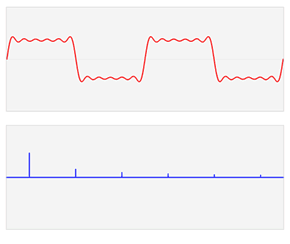
\includegraphics[width=0.5\textwidth]{assets/time-frequency.png}
	\end{figure}
		\subsubsection{Autocorrelation}
		A standard method of time-domain \f0 detection is autocorrelation. It exploits the fact that a periodic or quasiperiodic waveform such as a sustained sung note will be self-similar by the definition of periodicity. If we compare a waveform with a copy of that waveform offset by the period of the waveform i.e. \(\f0 ^{-1}\) then we should expect to see a strong correlation between them. So autocorrelation works by iterating over all the possible offset values, and determining which one has the best correlation. This correlation value for each different offset is described by the equation below, where x is the signal function, N is the window size of the waveform you are considering, and v is the offset value.  \[R_x(v) = \sum_{n=0}^{N-1-v} x[n]x[n+v]\]
		\subsubsection{Limitations}
		One fundamental limitation of Autocorrelation is that octave errors are frequently encountered. This occurs when the offset is calculated to be double what it should be, and is prone to happening as the nature of a periodic wave is such that if you shift it along twice the offset then you will also end up with a valid offset.
	
\section{Audio processing}



\chapter{Implementation}
\section{Web Application}
The program is taking the format of a web application with different musicality exercises on them. Users can pick and choose whatever exercises they would like to complete, which are grouped by category.
\subsection{Application flow}
	\subsubsection{Django web framework}
		\paragraph{Views}
		\paragraph{Models}
		Django interfaces with the database through Models. An example of this is the IntervalScore model below. This particular model stores all the information about a user's attempt at singing an interval in the interval training exercise.
		\begin{verbatim}
		class IntervalScore(models.Model):
   			interval = models.ForeignKey(Interval) 
    		timestamp = models.DateTimeField(auto_now_add=True)
    		score = models.FloatField();
		    user = models.PositiveIntegerField();
		    def __str__(self):
        		return " Score: " + str(self.score) + " for" + self.interval.name + " with user id: " + str(self.user)

		\end{verbatim}
		The interval field represents the interval that the user has attempted, the timestamp tells us when it was attempted, and the score field tells us the calculated score for that attempt (it will be explained how this metric is derived in "Measuring user ability")
		
\section{Pitch Detection}
\par Pitch detection is an important part of the exercises, and as such, robust pitch detection has been an important feature in the development of this program. 
\par Most existing pitch detection algorithms are based on real-time applications, i.e. where audio captured from a microphone is analysed and the pitch is displayed as a constantly updating function of the audio signal. This is useful for applications like guitar tuning, where you need near instant feedback, and you can be sure that the pitch you are inputting is fairly constant. 
\par With analysis of pitch in the human voice however, the problem is that even with well trained singers, the pitch of a note can vary quite considerable over a 2 second period, due to vibrato\footnote{Vibrato is the musical technique of intentionally oscillating the pitch of the note around a fixed point.}, or other causes that can be hard to pick up just by listening to yourself, so it is not always trivial to determine one pitch to summarise a sample of a single held note, and indeed, often not appropriate to do so if the singer cannot even stay on the same note for that short period of time, and wobbles around the note inconsistently.
\par It is with this in mind that I have developed a Segmented Pitch Detection Algorithm, that can accurately determine the pitch of a 2-3 second sample of singing.

\subsection{Segmented Pitch Detection Algorithm}
The principle of the Segmented Pitch Detection Algorithm is relatively simple: A given audio sample is split into several segments, pitch detection is run on each segment, and then the segments are analysed to calculate pitch.





\subsubsection{Choosing a segment size}
\par Most PC microphones sample audio at either 44,100Hz or 48,000Hz, as these ensure that the full 20KHz spectrum of human hearing can be recorded due to the Nyquist–Shannon sampling theorem (see Background section 2.5). For the sake of simplicity we will assume a sample rate of 48,000Hz for this report, though the program can handle either rate.
\par The human vocal range defined in section 2.4.2 was E2 - C6, which corresponds to a frequency range of ~80-1000hz\cite{scientificPitchTable}. To calculate the number of samples at either end of the range: 
 		 \[48000\div 96 = 600 \text{ samples}\] 
		 \[48000\div 1000 = 48 \text{ samples}\]
		
In order for our autocorrelation algorithm to work, it is  necessary to take a segment size at least twice that of the lowest frequency we wish to sample.
This is because in autocorrelation, we must compare the signal with an offset version of itself, and this score is maximal with an offset equal to the period of the signal. Therefore, in our example, if we use anything less than a 1200 sample size and are trying to detect a 96Hz signal, we won't even be able to autocorrelate on a full period. [DIAGRAM illustrating how you only compare half a period of you use a 900 sample segment] I have therefore decided to use 1200 as the segment size. Increasing this number results in a higher quality analysis per segment, but the trade-off is that segments per second decreases, meaning you are sacrificing granularity of change of pitch over time. [DIAGRAM of debug freqs graph at differing window sizes.
		
\section{Measuring user ability}
Discussion of the measuring of user ability for the various different exercises.
\section{Adapting to user ability}
Discussion of the adaptive element of the program for different exercises.
\section{Exercises}


\chapter{Evaluation}

In order to evaluate the success of my program, I have used both qualititative and quantitative methods which I will outline in the chapter.

\section{Adaptivity}
How well I have achieved adaptivity in my teaching will be a difficult thing to test quantitatively, as there is no existing way of measuring how adaptive a learning system is. One way to gain a greater understanding of how effective the adaptivity is would be to use the program and artificially fail parts of exercises to try and prompt the system to adapt to my behaviour, and see how it responds.

\section{Intuitiveness}
The intuitiveness of my program is something that can only be judged by other people using it. I intend to involve others in the design process from the start, by using techniques like hallway testing to quickly get feedback on how users approach my app, and what they would change about it. At the end of the project I will also hopefully get as many different people as I can to use it, and fill in a survey at the end of their usage period detailing their experience with the app.
\section{User Engagement}
This will be handled by users answering questions about whether they would continue using it, and how much they enjoyed the process. These questions will be found on the survey described above.

\section{Teaching Proficiency}
To measure the general success of my product as a teaching tool, I shouldn't actually have to do too much, as (if succesfully implemented), my app should be able to track the users progress, and store information about how much they've improved.

\section{Pitch Detection}
I have developed a test set for my pitch detection algorithm. This consists of multiple different samples of 1 or 2 seconds of a note being sung at a specific  known pitch. I have included samples from many different people in my test set to make sure my pitch detection works for as many different voice types as possible. I have also recorded people using a very basic microphone used on my laptop, so I can ensure that the pitch detection will work even with fairly low quality audio. 

Here are the results of what I found...

following sections includes pictures of my pitch detection output, as well as percentage correct results for my algorithm.
\chapter{Conclusions}
This chapter summarises the achievement of this project, as well as pointing out ideas for future work.

Adaptive learning in the context of music education is an unexplored field, as adaptive learning is still a growing field itself. In this project, I have devised a computer application that provides an adaptive learning experience for intonation training using a segmented autocorrelation algorithm. 
Initially, I hoped to include several different exercises that would test a wide variety of musical skills, however, I have only managed to get the intonation exercise up and running.
The exercise itself is, I believe, a successful one, and one unlike anything else existing. 
Adaptive learning has been successfully implemented in this exercise, and when a user spends time on it, they will find that it changes to match their ability.
The pitch detection algorithm is highly successful and reliable, and it has shown that it can cope with variable levels of background noise.



\section{Future}
Though the project is finished, there is much more that could be done to enhance and extend it. \begin{itemize}
	\item A greater variety of exercises. At present, the only exercise available to the user is interval training. There are many different exercises that could work in an adaptive learning context, for example, the rhythmical exercise mentioned in the background.
	\item A melody analyser. The pitch detection algorithm is nearly sufficiently sophisticated as to be able to detect pitch in samples containing melodies. This would be an interesting feature that could pave the way for automated music dictation.

\end{itemize}
\include{./appendix}

\bibliographystyle{ieeetr}
\bibliography{master}

\end{document}
